\documentclass[conference]{IEEEtran}
\usepackage[utf8]{inputenc}
\usepackage{amssymb}
\usepackage{amsmath}
\usepackage{graphicx}
\usepackage{amsthm}
\usepackage{hyperref}
\usepackage{algorithm}
\usepackage{algorithmic}
\usepackage{authblk}
\usepackage{subcaption}
%\usepackage{natbib}

\hyphenation{AdaBoost}

\DeclareMathOperator{\margin}{margin}
\DeclareMathOperator{\sign}{sign}
\DeclareMathOperator{\conf}{conf}
\DeclareMathOperator{\argmin}{argmin}
\newtheorem{definition}{Definition}
\newtheorem{theorem}{Theorem}

\title{A Confidence-Based Approach for Balancing Fairness and Accuracy}
\author{submitted for blind review}

\begin{document}

\maketitle

\begin{abstract} 

We study three classical algorithms in the context of fairness: adaptive
boosting, support vector machines, and logistic regression.  Our goal is to
maintain the high accuracy of these learning algorithms while reducing the
degree to which they discriminate against individuals because of their
membership in a certain protected group.  A common feature of these learning
algorithms is that one can easily measure their confidence in the
classification of a point.  Our main contribution is a method for achieving
fairness by shifting the confidence threshold for the protected group.  We
compare this method with other ``fair'' variants of these learning algorithms
as well as results in previous papers in the fairness literature.  Our method,
in addition to outperforming the state of the art in terms of achieving high
accuracy and low discrimination, also allows for a fast and simple
quantification of the trade-off between bias and error.  We study this
trade-off for all three methods on three different datasets.  We further define
a new notion of fairness by introducing a modeling assumption on the process
generating bias in the training data, and we evaluate our methods according to
this measure. 

\end{abstract}

Machine learning algorithms assume an increasingly large role in making
decisions across business and government. This has naturally raised concerns
about discrimination encoded in training data, which is subsequently learned by
algorithms to perpetuate discriminatory decisions against groups that are
protected by law, even in the absence of ``discriminatory intent'' by those
designing and deploying the algorithm. A typical example is an algorithm
serving potentially predatory ads to protected groups. Such issues resulted in
a 2014 report from the US Executive Office~\cite{PodestaPMHZ14} which voiced
concerns about discrimination in machine learning and called for additional
research to design fair algorithms.  The primary question we study in this
paper is

\begin{center}
How can we maintain high accuracy of a learning algorithm while reducing
discriminatory biases?
\end{center}

The measure of fairness we consider is \emph{statistical parity}, which is
achieved by definition if the protected subgroup is as likely as the
unprotected population to have a given label. As one would expect, if the
training data provided to a learning algorithm encodes bias then any success in
removing that bias incurs some cost in the classifier's accuracy. Hence, a
primary concern is to study the trade-off between bias and accuracy and design
algorithms that make favorable trade-offs. 

An approach to optimizing this tradeoff is to identify examples for which the
learning algorithm is ``unsure'' of the correct classification, and manipulate
the labels of these points so as to improve fairness. Indeed, by changing the
labels of ``unsure'' examples, we can reduce bias and still maintain low error
rate, and we show this is the case for three famous learning algorithms:
AdaBoost, support vector machines, and logistic regression. Each algorithm
provides a measure of confidence in its prediction which we leverage to improve
the fairness of the final classification. While we compare a few potential
methods for reducing bias, our most successful method uses the confidence
values to ``shift the decision boundary'' for members of the protected class.
This technique achieves or outperforms the state of the art on the datasets we
test.  These datasets provide both a natural interpretation of the method and a
quantification of the error-bias tradeoff.

A major challenge in the study of fairness in learning is to find an
appropriate definition of what it means for an algorithm to be fair.
Presently there is no single accepted definition of fairness.
Dwork~et~al.~\cite{DworkHPR12} point out that statistical parity is only a
measure of population-wide fairness. In particular, they provide a laundry list
of ways one could achieve statistical parity while still exhibiting serious and
unlawful discrimination.  In addition to analyzing the statistical parity of
our methods, we introduce a new notion of fairness that we call \emph{random
bias individual fairness} (RBIF). Intuitively, this measure assumes the bias is
generated i.i.d. at random, and measures the ability for the learning algorithm
to recover the true labels when given the biased training data. We produce
unbiased data by generating a new random feature for a given dataset, and then
we introduce synthetic bias against that feature.

Although there are several papers on ``fair'' versions of learning algorithms
such as naive Bayes and decision trees, some of the most successful and widely
used machine learning algorithms have not been studied in the context of fair
learning before. In this paper we consider three ubiquitous learning
algorithms: boosting, support vector machines, and logistic regression.
Fairness properties of logistic regression have been studied previously by
Kamashima et. al~\cite{KamashimaAS11}; to the best of our knowledge we are the
first to study boosting and SVM in this context, and our confidence-based
analysis is new for all three algorithms. 

The paper is organized as follows. In Section~\ref{sec:background} we review
the previous work on fairness and the three algorithms we study.
In Section~\ref{sec:methods} we define four methods for fair learning as well
as \emph{random bias individual fairness}.  In Section~\ref{sec:experiments} we
describe our experiments and their results.\footnote{The entire Python source
used to generate the diagrams and tables is available at
\url{https://www.dropbox.com/sh/p7s6nghntvdxxeo/AABJQIhaH_GDIZJnYAurgufpa?dl=0}.
This will be updated to a (non-anonymized) Github repository for the final
version.}  We close with a discussion in Section~\ref{sec:discussion}.
 

\section{Background} \label{sec:background}

\subsection{Notions of fairness} 

The study of fairness in machine learning is young, but there has been a lot of
disparate work studying notions of what it means for data to be fair. See the
extensive survey of~\cite{RomeiR14} for a detailed discussion. Still, there is no
established measure of \emph{fairness} for a learning algorithm. Two
prominent definitions of fairness that have been recently studied in the
literature are \emph{statistical parity} and \emph{$k$-nearest-neighbor
consistency.}

\emph{Statistical parity:} Let $D$ be a distribution over a set of labeled
examples $X$ with label $l : X \to \{-1, 1\}$ and a protected subset $S \subset
X$. The \emph{bias} of $D$ is defined as the difference in probability of an
example in $S$ having label 1 and the probability of an example in $S^C$ having
label 1, i.e.

$$ 
   B(D, S) = \Pr_{x \sim D|_{S^C}}[l(x) = 1] - \Pr_{x \sim D|_{S}}[l(x) = 1].
$$

The bias of a hypothesis $h$ is the same quantity with $h(x)$ replacing $l(x)$.
If a hypothesis has low bias in absolute value we say it achieves
\emph{statistical parity.} Note that $S$ represents the group we wish to
protect from discrimination, and the bias represents the degree to which they
have been discriminated against.  The sign of bias indicates whether $S$ or
$S^C$ is discriminated against. We use statistical parity for our
population-wide fairness measure.

\emph{$kNN$-consistency:} Dwork et al. \cite{DworkHPR12} point out that while
bias is undesirable, it does not account for all possible forms of
discrimination.  Rather, it is a measure of group fairness rather than
individual fairness. The second notion, due to~\cite{DworkHPR12}, calls a
classifier ``individually fair'' if it classifies individuals who are close to
each other similarly. They use $k$-nearest-neighbor to measure consistency of
close individuals. Note ``closeness'' is defined with respect to a metric space
chosen as part of the data cleaning and feature selection process. 

We define a new notion of fairness that departs from previous literature in
that it does not require a metric on the underlying space. Rather, it makes the
assumption that the process generating the bias is i.i.d. random, and measures
the ability for an algorithm to recover the true labels from the biased
dataset. We posit that any algorithm which is considered ``fair'' should
recover from i.i.d. random bias against a protected class.

\emph{Other fairness measures:} 
Friedler et al.~\cite{FriedlerSV14} define a measure called \emph{disparate
impact} based on the ``$80\%$ rule'' used by some US government institutions
and present approaches to reduce it.  For more information on different notions
of discrimination and fairness of data, we refer the reader to the survey of
Romei and Ruggieri~\cite{RomeiR14}.

\subsection{Related work on fair algorithms}
Learning algorithms studied previously in the context of fairness include naive
Bayes~\cite{CaldersV10}, decision trees~\cite{KamiranCP10}, and logistic
regression~\cite{KamishimaAAS12}.  The two main approaches in most of these
papers are massaging and regularization. Massaging means changing the biased
dataset before training to remove the bias in the hope that the learning
algorithm trained on the now unbiased data will be fair.  Massaging is done
in the previous literature based on a ranking learned from the biased data.  In
this paper we do massaging randomly for the sake of simplicity.  The
regularization approach consists of adding a regularizer to the optimization
problem which penalizes the classifier for discrimination.

Two other notable papers in the fairness literature are ``Fairness through
awareness'' (\cite{DworkHPR12}) and ``Learning Fair Representations''
(\cite{ZemelWSPD13}).  In the former paper the authors describe a framework for
maximizing the utility of a classification with the constraint that similar
people be treated similarly. One shortcoming of this approach is that it relies
on a hypothetical metric on the data that tells us the similarity of
individuals with respect to the classification task. As the authors themselves
admit, it is unclear how such a metric can be obtained.  The authors of the
latter paper formulate the problem of fairness in terms of intermediate
representations: the goal is to find a representation of the data which
preserves as much of the relevant attributes of the original data points as
possible while simultaneously obfuscating membership in the protected class.

When applicable, we will include the results of the earlier papers for
comparison.


\subsection{AdaBoost}

Boosting algorithms work by combining \emph{base hypotheses}, ``rules of
thumb'' that have a fixed edge over random guessing, into highly
accurate predictors.  In each round, a boosting algorithm will change the
weights of the data points and find the base hypothesis that achieves the
smallest weighted error on the sample.  It always increases the weights of the
incorrectly classified examples, thus forcing the base learner to improve the
classification of the examples that are the hardest to classify correctly. In
this paper we study AdaBoost, a ubiquitous boosting algorithm.  The
algorithm is given in Algorithm~\ref{adaboost}.  In all of our experiments we
boost decision stumps for $T=20$ rounds. 

\begin{algorithm}
\caption{AdaBoost \cite{FreundS97}}
\begin{algorithmic}\label{adaboost}
\FOR {$i=1$ \TO $m$}
\STATE $D_1(i) = \frac1m$
\ENDFOR
\FOR {$t=1$ \TO $T$}
\STATE $h_t = $ base hypothesis with smallest error
\STATE $\epsilon_t = \sum_{i=1}^m D_t(i) (1-\delta_{h_t(\mathbf x_i), y_i})$
\STATE $\alpha_t = \frac12\log\frac{1-\epsilon_t}{\epsilon_t}$
\STATE $Z_t = 2\sqrt{\epsilon_t (1-\epsilon_t)}$
\FOR {$i=1$ \TO $m$}
\STATE $ D_{t+1}(i) = \frac{D_t(i) e^{-h_t(\mathbf x_i) y_i}}{Z_t}$
\ENDFOR
\ENDFOR
\STATE $g=\sum_{t=1}^T \alpha_t h_t$
\STATE $h = \mathrm{sgn}\circ g$
\RETURN $h$
\end{algorithmic}
\end{algorithm}

Given hypotheses $h_i$ with weights $\alpha_i$ computed by AdaBoost, the
\emph{margin} of a labeled data point $(\mathbf x,y)$ is

$$ \margin(\mathbf x,y) = y\frac{\sum_{i=1}^T \alpha_i h_i(\mathbf
x)}{\sum_{i=1}^T \alpha_i}$$

where $\alpha_i$ is the weight of $h_i$ in the linear combination defined by
AdaBoost.  We define the similar \emph{signed confidence} of AdaBoost for an
unlabeled point $x$,

$$ \conf(\mathbf x) = \frac{\sum_{i=1}^T \alpha_i h_i(\mathbf x)}{\sum_{i=1}^T \alpha_i}.$$

The absolute values of the two quantities are equal and measure the confidence
of AdaBoost in its classification for that particular example.  The difference
between the two is that whereas the sign of the margin indicates whether the
classification is correct, the sign of the confidence tells us the
classification itself. Also, the signed confidence can be computed without
access to the correct label.

It is well known that the training error of AdaBoost decreases exponentially in
the number of rounds, and Schapire et al.~\cite{SchapireFBL98} prove that the
generalization error of AdaBoost can be bounded in terms of the empirical
probability of observing a small value of $\margin(\mathbf x)$ on the training set.
This suggests that examples with small confidence are more likely to be
incorrect than examples with large margins. In particular, one might hope that
one could take advantage of this for fairness by flipping negative labels of
members of the protected class with a small confidence. Indeed, is the strategy
we analyze in the rest of this paper.

\subsection{Support vector machines}

The support vector machines is a framework for learning linear predictors in
high (possibly even infinite) dimensional feature spaces.  A hyperplane is
defined by its normal vector $\mathbf w$.  If positive and negative examples
are separable by a hyperplane, the hyperplane with the largest margin, i.e. the
largest distance from the nearest point, is returned.  Often the rather strong
assumption of linear separability does not hold.  In this case we solve a
regularized loss minimization problem introduced by Cortes and
Vapnik~\cite{CortesV95} and commonly called Soft-SVM:

$$\min_{\mathbf w,\mathbf \xi, b} \left(\frac12\|\mathbf w\|^2+C\sum_{i=1}^m \xi_i\right)$$
$$\textnormal{s.t. } \forall i: y_i(\mathbf w\cdot \mathbf x_i +b)\ge 1-\xi \textnormal{ and } \xi_i\ge 0.$$

We will also use the kernel trick, introduced by Boser et al.~\cite{BoserGV92},
of implicitly embedding the input space into some higher dimensional feature
space.  The embedding is defined by a symmetric positive semidifinte function
$K(\mathbf x,\mathbf x')$ corresponding to the inner product of the space. In
this paper we will use the Gaussian (RBF) kernel $K_{RBF}(\mathbf x,\mathbf x')
=\mathrm{exp}\left(-\frac{\|\mathbf x-\mathbf x'\|^2}{2\sigma^2}\right)$ with
parameter $\sigma=0.1$ for the Census Income and Singles datasets and the
linear kernel $K_{lin}(\mathbf x,\mathbf x') =\langle\mathbf x,\mathbf
x' \rangle$ for the German dataset (the datasets are described in
Section~\ref{sec:experiments}).  The kernel function defines an embedding
$\psi$ from the input space into an infinite-dimensional Hilbert space.  Let
$\mathbf w$ denote the normal vector of the hyperplane found by the kernelized
SVM in this space.  Then we define the \emph{confidence} of SVM as follows:
$$\conf(\mathbf x) = \langle \mathbf w, \psi(\mathbf x)\rangle.$$ As in the
case of boosting, the confidence has the same magnitude as the analogous SVM
margin, but the sign indicates the classification instead of its correctness.

\subsection{Logistic regression}

Logistic regression is also a method for learning linear predictors.  The
classifier output by logistic regression is of the form

$$h(\mathbf x)=\sign(\phi(\langle \mathbf w, \mathbf x\rangle) - 1/2)$$

where $\phi(z)=\frac{1}{1+e^{-z}}$ is the logistic function. The vetor $\mathbf
w$ is found by empirical risk minimization. The loss function used in logistic
regression is the logistic loss

$$\ell(\mathbf w, (\mathbf x,y))=\log(1+e^{-y\langle \mathbf w, \mathbf x\rangle}).$$

The ERM problem associated with regularized logistic regression is 
$$
   \argmin\limits_{\mathbf w} \|\mathbf w\|^2+ C 
      \sum_{i=1}^m \log(1+e^{-y_i\langle \mathbf w, \mathbf x_i\rangle}).
$$
Here we define the confidence of logistic regression simply as the value that
the classifier takes before rounding:
$$\conf(\mathbf x) = \phi(\langle \mathbf w, \mathbf x\rangle).$$
\section{Methods} \label{sec:methods}

We define our methods. In what follows $X$ is a labeled dataset, $l(x)$ are the
ground truth labels, and $S \subset X$ is the protected group.  We further
assume that members of $S$ are less likely than $S^C$ to have label 1.  First
we describe three relabeling algorithms.  A relabeling algorithm, when given a
hypothesis $h$ and a labeled data set $(X, l)$, produces a new hypothesis $h'$
that flips the output of $h$ according to some rule.

The \emph{random relabeling} (RR) algorithm computes the probability
$p$ for which, if members of $S$ with label $-1$ under $h$ are flipped by $h'$
to $+1$ randomly and independently with probability $p$, the bias of $h'$ is
zero in expectation. The classifier $h'$ is then defined as the randomized
classifier that flips members of $S$ with label $-1$ with probability $p$ and
otherwise is the same as $h$.

Next, we define \emph{random massaging} (RM).  Massaging strategies, introduced
by~\cite{KamiranC09}, involve eliminating the bias of the training data by
modifying the labels of data points, and then training a classifier on this
data in the hope that the statistical parity of the training data will
generalize to the test set as well.  In our experiment, we massage the data
randomly; i.e.~we flip the labels of $S$ from $-1$ to $+1$ independently at
random with the probability needed to achieve statistical parity in
expectation, as in RR.

Our main contribuition is the following algorithm which we will call
\emph{shifted decision boundary} (SDB).  This is a relabling algorithm which
takes confidence into consideration.  The classification of a data point by any
of the three learning algorithms studied in this paper is a function of the
confidence: the predicted label is positive if and only if the confidence is
above a fixed threshold. This threshold is $0$ for AdaBoost and SVM and
$\frac12$ for logistic regression.  Also, for these algorithms, the
classification is more likely to be correct for data points with high absolute
confidence. Consequently by changing the labels of data points in the
protected group which have small negative confidence, not only do we reduce
bias, but we likely do not increase label error significantly since these
points are likely to be misclassified by $h$.  Relabeling points with small
negative confidence is equivalent to shifting the confidence threshold down:
indeed, this is what our algorithm will do for points in the protected group.

More formally, the SDB algorithm computes the value $\theta$ such that bias is
minimized by shifting the minimum required signed confidence for examples from
$S$ from zero to $\theta$. That is, SDB returns a classifier $h'$ of the following form: $x \in S$ then $h'(x) = 1$ iff $\conf(x)
\ge \theta$, and otherwise $h'(x) = h(x)$.  Then $\theta$ is chosen to minimize the bias of $h'$ on $S$.

Finally, in \emph{fair weak learning} (FWL) we replace a standard boosting weak
learner with one which tries to minimize a linear combination of error and bias
and run the resulting boosting algorithm unchanged. The weak learner we use
computes the decision stump which minimizes the sum of label error and bias of
its induced hypothesis. Fair weak learning is only applicable to boosting.

Now we define our new method for evaluating the fairness of an algorithm.  As
we noted in Section~\ref{sec:background}, previous notions of fairness all
suffer from one of the following two problems: either they only measure
fairness in statistical terms over the entire group or, if they aim to measure
individual fairness, they rely on additional information about the data (such
as a metric) which is usually not available explicitly.\footnote{Moreover, the
work in~\cite{DworkHPR12} suggests that learning a suitably fair similarity
metric from the data is as hard as the original problem.}

To construct a fairness measure that does not suffer from these limitations, we
introduce synthetic bias to the data. The advantage of synthetically generated
bias is that in this case we know the original, unbiased ground truth, and
therefore we can measure the performance of the learning algorithm against this
ground truth. In addition, we guarantee by design that we avoid the adversarial
targeted discrimination types listed in~\cite{DworkHPR12}.

In particular, we test how these algorithms are resistant to random noise that
introduces bias against a random subset of the individuals.  This is formalized
as follows:

\begin{definition}
We define the \emph{random bias individual fairness} (RBIF) of a learning
algorithm $A$ on a labeled dataset $X,l$ as follows. Introduce a new uniformly
random binary feature $z$ on elements of $X$. Flip the labels of examples $x$
that have $z=0$ independently with probability $p$ to $-1$ to get a new dataset
$X', l'$. Run $A$ on $X', l'$ and let $h$ be the resulting hypothesis. The
random bias individual fairness of $A$ is the expected fraction of flipped
examples $x \in X'$ for which $h(x) = l(x)$.  
\end{definition}

In our experiments we set $p = 0.2$.  RBIF can be thought of as the following
experiment:  A learning algorithm is given a dataset in which bias has been
generated at random.  That is, we change the labels of a few individuals based
on a feature which is random with respect to the classification task.  The goal
of the algorithm is to then recover the ground truth labels in the original
dataset.  This models the probability that an individual who is subject to
random bias will be treated fairly.

This definition naturally generalizes to an arbitrary distribution over
examples, and we defer the analysis of such a definition to future work. 

\section{Experiments} \label{sec:experiments}

\subsection{Datasets}

The Census Income dataset~\cite{Lichman13}, extracted from the 1994 Census
database, contains demographic information about $48842$ American adults.  The
prediction task is to determine whether a person earns over \$50K a year.  The
dataset contains $16,192$ females ($33\%$) and $32,650$ males. Note $30.38\%$
of men and $10.93\%$ of women reported earnings of more than \$50K, therefore
the bias of the dataset is $19.45\%$. Further note that since $76\%$ of the
data points have negative labels, the constant $-1$ classifier achieves $76\%$
accuracy and perfect statistical parity. This baseline does not appear to have
been considered in previous literature for fair algorithms which used this
dataset.

\begin{figure}[t]
\centering
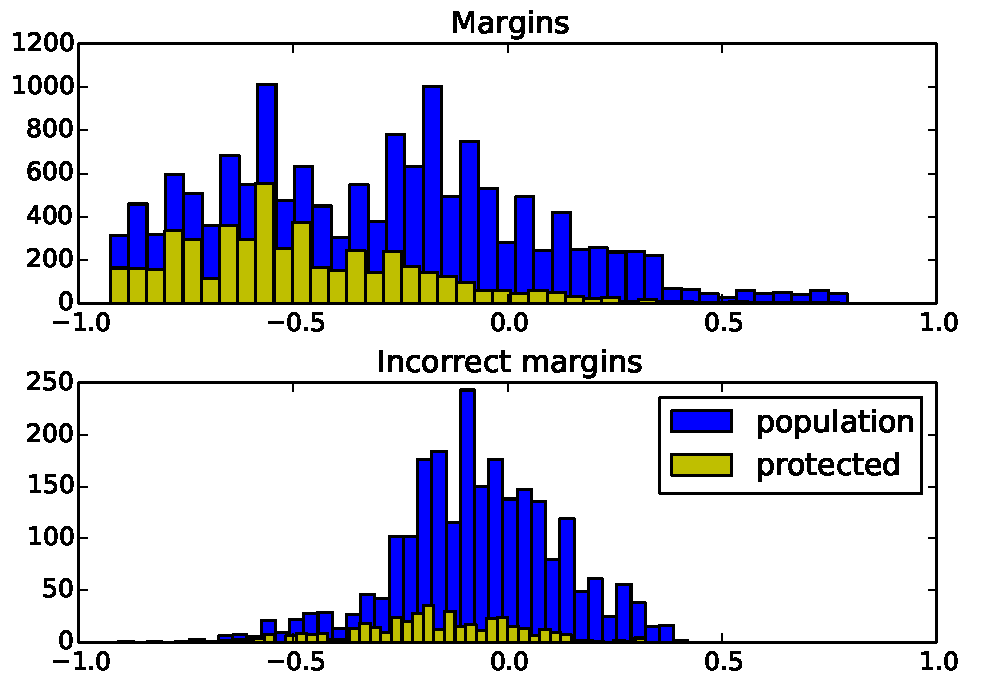
\includegraphics[width=\columnwidth]{images/censusmargins.pdf}
\caption{Histogram of boosting confidences for the Census data set. The vast
majority of women are classified as $-1$, and the incorrect classifications are
closer to the decision boundary.}
\label{fig:boosting-margins}
\end{figure}

The German credit dataset~\cite{Lichman13} contains financial information about
1000 individuals who are classified into groups of good and bad credit risk.
The ``good'' credit group contains $699$ individuals. Following the work
of~\cite{KamiranC09}, we consider age as the protected attribute with a cut-off
at $25$. Only $59\%$ of the younger people are considered good credit risk,
whereas of the $25$ or older group, $72\%$ are creditworthy. This gives us a
bias of $13\%$.

In the Singles dataset, extracted from the marketing dataset
of~\cite{HastieTF09}, the goal is to predict whether annual income of a
household is greater than \$25K from 13 other demographic attributes.  The
protected attribute is gender.  The dataset contains $3,653$ data points,
$1,756$ ($48\%$) of which belong to the protected group. $34\%$ of the dataset
has a positive label.  We extracted the subset of records whose respondents
identified as ``single.''

\subsection{Results and analysis}\label{sec:results}

In this section we state our experimental results. They are summarized in
Tables~\ref{table:census_results},~\ref{table:german_results},
and~\ref{table:singles_results} for the Census Income, German, and Singles
datasets, respectively.  For comparison, we also included the numbers for the
Learning Fair Representations (LFR) method of~\cite{ZemelWSPD13} for the Census
Income dataset and also the numbers for the Classification with No
Discrimination (CND) method of~\cite{KamiranC09} (these numbers were estimated
from figures in the paper since they were reported graphically). In the
former paper, the authors implemented three other learning algorithms, these
are unregularized logistic regression, Fair Naive-Bayes \cite{KamiranC09}, and
Regularized Logistic Regression \cite{KamashimaAS11}.  These methods all had
errors above $20\%$; thus we see that our confidence-based relabeling methods
outperform the state of the art for the Census Income dataset.  To investigate
the trade-offs made by these relabeling methods more closely,
Figures~\ref{fig:adult_tradeoffs},~\ref{fig:german_tradeoffs},
and~\ref{fig:singles_tradeoffs} show the rate at which error increases as bias
goes to zero.

For the Census Income dataset, AdaBoost and logistic regression with SDB have
the best performance. Both SDB algorithms achieve statistical parity with
about $18\%$ error. Logistic regression with RM achieves slightly lower error
($17.96\%$) with $-2.25\%$ bias.  Moreover, the two SDB algorithms have the
highest RBIF. To the best of our knowledge, no other published method has
achieved statistical parity with less than $20\%$ error.

The different methods have similar performance on the German dataset with
accuracy mostly in the $24$-$27\%$ range. Variants of logistic regression have
the smallest error. As Figure~\ref{fig:german_tradeoffs} shows, label error
practically stays constant as the decision boundary is shifted.

In the case of the Singles dataset, SDB for SVM is the clear winner. It is
notable that not only is there no significant increase in the error compared to
the unmodified SVM baseline, but error actually decreases slightly as the
confidence threshold is shifted for the protected group. (This can also be seen
in Figure~\ref{fig:singles_svm_tradeoff}.)

Note again the difference in SVM kernels between the datasets.  The Gaussian
kernel performs well for the Census Income and Singles dataset.  However, in
the case of the German dataset, which is the smallest of the three, with the
Gaussian kernel every point becomes a support vector. This is not only a clear
sign of overfitting but also makes SDB impossible since the model gives the
same confidence for almost every data point.

We found that fair weak learning (FWL) does empirically reduce bias, but does
not achieve statistical parity.  Moreover, the label error of FWL is not better
than that of SDB, and the trade-off between label error and bias cannot easily
be controlled. The same is true for random massaging. On the other hand, we can
see from Table~\ref{table:german_results} that at least in some cases RM and
FWL perform equally well with SDB, though in most cases one or both methods are
far worse.

A further advantage of SDB is that the trade-off between label error and bias
can be controlled after training.  To decide how much bias and error we want to
allow, we do not have to pick a hyperparameter before training the algorithm,
unlike for most other fair learning methods. This means that the computational
cost of choosing the best point on the trade-off curve is very low, and the
tradeoff is transparent. These results show the advantages of SDB: the
confidence can be used to find a superior classifier.

The results also show the usefulness of RBIF as a measure of fairness.  As we
can see in Tables~\ref{table:census_results} and~\ref{table:singles_results},
even when random relabeling slightly outperforms SDB in terms of label error,
SDB often beats RR by as much as ten percent RBIF. This suggests that the
performance of fair learning algorithms should not be evaluated solely by their
accuracy and bias.

A natural baseline for RBIF is $0.5$, since a hypothesis chosen uniformly at
random will flip back half of the points that were flipped to $-1$.  We see
that the RBIF of the unmodified learning algorithms, with the exception of SVM
and AdaBoost on the German dataset, is almost always below $0.5$, showing that
the classifiers encode the bias introduced into the training data.  Our
evidence that we can recover from randomly introduced bias while still
achieving low label error is promising. Even though the RBIF of the fair
learning algorithms is often still below $0.5$, they increase RBIF
significantly compared to the unmodified baseline, sometimes almost doubling
it.

\section{Discussion}\label{sec:discussion}

In this paper, we introduce a general method for balancing discrimination and
label error. This method, which we call shifted decision boundary (SDB),
is applicable to any learning algorithm which has an efficiently computable
measure of confidence. We study three such algorithms, AdaBoost, SVM, and
linear regression, compare our methods to other methods proposed in the
earlier literature and our own baselines, and empirically evaluate our
methods' performance on three datasets. We find that SDB generally outperformed
our other methods and the state of the art, and we provide theoretical justification
for its success. 

We define the RBIF measure, and our empirical results suggest its usefulness in 
measuring an algorithm's fairness. Although i.i.d. random bias is a simplified
and admittedly unrealistic model of real-world discrimination, we posit that
any algorithm which can be considered fair must be fair with respect to RBIF.
Moreover, RBIF generalizes to an arbitrary distribution over the input data. We
leave the theoretical analysis of this generalization to future work.

Finally, we have not analyzed measures such as SDB and RBIF from a legal or
sociological perspective. Despite achieving low bias and high accuracy, SDB
generalizes (and can be interpreted as) ``lowering the bar'' for the protected
class. Such methodologies are controversial in practice, and it is not clear to
what extent shifting a decision boundary of a learning algorithm, which may be
composed of a complex combination of features, constitutes ``lowering the
bar.'' Likewise, it would be interesting to relate RBIF to legal notions of
fairness.


% !!! REMOVED FOR TRIPLE-BLIND REVIEWING, SHOULD BE ADDED TO CAMERA-READY VERSION
% \section*{Acknowledments}
% We would like to thank Lev Reyzin for helpful discussions.

\begin{table*}
\centering
\begin{tabular}{| c | ccccc |}
\hline
               & SVM & SVM (RR) & SVM (SDB) & SVM (RM) & LFR \cite{ZemelWSPD13} \\
\hline 
label error    & 0.1471 (3.2e-33)  & 0.2006 (2.9e-06) & 0.2198 (0.0) & 0.1749 (7.1e-06) & 0.2299 \\ 
bias           & 0.1689 (3.2e-33)  &  -0.0179 (2.1e-05) &  -0.1550 (8.5e-34) & 0.0713 (8.2e-05) & 0.0020 \\ 
RBIF           & 0.2702 (2.0e-04) & 0.2821 (2.0e-04) & 0.2925 (2.0e-04) & 0.2706 (2.2e-04) & n/a \\ 
\hline
               & LR & LR (RR) & LR (SDB) & LR (RM) & \\
\hline 
label error    & 0.1478 (2.3e-07)  & 0.2056 (4.7e-06)  & 0.1828 (4.1e-6) & 0.1796 (1.8e-05) & \\ 
bias           & 0.1968 (1.1e-05) & -0.0046 (3.3e-05)  & -0.0068 (2.0e-5) &  -0.0225 (3.0e-04) & \\ 
RBIF           & 0.4647 (1.7e-04)   & 0.4637 (5.9e-04) & 0.5554 (4.9e-04) & 0.4361 (2.0e-04) &  \\ 
\hline
               & AdaBoost & AB (RR)  & AB (SDB)  & AB (RM)   & AB (FWL)  \\
\hline 
label error    & 0.1529 (4.8e-06)  & 0.2073 (1.2e-05)  & 0.1828 (1.4e-05) & 0.1888 (5.3e-05) & 0.1820 (3.6e-05)\\ 
bias           & 0.1856 (1.4e-04)  &  -0.0025 (3.8e-05) &  -0.0036 (1.4e-05) & -0.0283 (1.5e-03) & 0.0691 (0.0001) \\ 
RBIF           & 0.4372 (1.0e-03)  & 0.4645 (3.2e-04)  & 0.5340 (9.4e-04) & 0.421 (6.8e-04) & 0.5174 (0.0004) \\ 
\hline
\hline 
\end{tabular}
\caption{A summary of our experimental results for the Census Income data for relabeling, massaging, and
the fair weak learner. The threshold for SDB was chosen to achieve perfect
statistical parity on the training data.  The variances are in parentheses.}
\label{table:census_results}
\end{table*}

\begin{table*}
\centering
\begin{tabular}{| c | ccccc |}
\hline
               & SVM & SVM (RR) & SVM (SDB) & SVM (RM) & CND \cite{KamiranC09} \\
\hline 
label error    & 0.2823 (0)      & 0.2802 (2.2e-05)   & 0.2742 (0.00073) & 0.2784 (0.00015) & 0.2757 (0.026) \\ 
bias           & 0.0886 (1.8e-33)& -0.0302 (0.0015)   & -0.0530 (0.0014)  & -0.0821 (0.00099) & 0.0327 (0.0020)  \\ 
RBIF           & 0.6756 (0.0065) & 0.8218 (0.0059)   & 0.8011 (0.0095)  & 0.6401 (0.0097) & n/a  \\ 
\hline
               & LR & LR (RR) & LR (SDB) & LR (RM) &  \\
\hline 
label error    & 0.2541 (2.1e-05)  & 0.2489 (3.7e-05)  & 0.2538 (0.00016) & 0.2495 (8.5e-05) &\\ 
bias           & 0.1383 (0.0002)  & -0.0605 (0.0020)  & -0.0942 (0.0016) & -0.1006 (0.00066) &\\ 
RBIF           & 0.3070 (0.0045)  & 0.8791 (0.0024)  & 0.8659 (0.0032) & 0.6599 (0.0034) & \\ 
\hline
               & AdaBoost & AB (RR)  & AB (SDB)  & AB (RM)   & AB (FWL)  \\
\hline 
label error    & 0.2602 (8.3e-05)  & 0.2589 (0.00019)  & 0.2622 (0.00032) & 0.2576 (0.00016) & 0.2520 (0.0001)\\ 
bias           & 0.2617 (0.0074)  & -0.0310 (0.0022)  & -0.0539 (0.0025) & 0.0211 (0.0042) & 0.2355 (0.0084)  \\ 
RBIF           & 0.6774 (0.0048)   & 0.8854 (0.0048)  & 0.8406 (0.0065) & 0.6633 (0.0040) & 0.6935 (0.0069) \\ 
\hline
\hline 
\end{tabular}
\caption{A summary of our experimental results for the German data for relabeling, massaging, and
the fair weak learner. The threshold for SDB was chosen to achieve perfect
statistical parity on the training data.  The variances are in parentheses.}
\label{table:german_results}
\end{table*}

\begin{table*}
\centering
\begin{tabular}{| c | ccccc |}
\hline
               & SVM & SVM (RR) & SVM (SDB) & SVM (RM) & \\
\hline 
label error    & 0.2718 (3.2e-33)& 0.2919 (1.5e-05)   & 0.2672 (5.3e-05) & 0.2750 (1.7e-04) & \\ 
bias           &0.0550 (2.0e-34)& 0.0311 (1.3e-04)  & 0.0039 (4.4e-04) & 0.0209 (8.4e-04) & \\ 
RBIF           &0.2424 (2.0e-03)& 0.2931 (1.8e-03) & 0.3016 (9.7e-04) & 0.2175 (2.2e-03)  &\\ 
\hline
               & LR & LR (RR) & LR (SDB) & LR (RM) &  \\
\hline 
label error    & 0.2742 (1.3e-32)  & 0.3165 (3.6e-05) & 0.2850 (7.2e-05)& 0.2824 (7.3e-06)&\\ 
bias           & 0.1468 (1.0e-34)  & 0.0054 (2.5e-04)  & -0.0090 (2.7 e-04) & 0.0556 (9.6e-05) &\\ 
RBIF           & 0.1971 (1.3e-03) & 0.2603 (1.3e-03)  & 0.3606 (4.6e-03) & 0.1905 (3.0e-03) & \\ 
\hline
               & AdaBoost & AB (RR)  & AB (SDB)  & AB (RM)   & AB (FWL)  \\
\hline 
label error    & 0.2690 (1.4e-05)  &0.2914 (1.1e-04)  & 0.2762 (6.5e-05) & 0.2713 (5.3e-06) & 0.2705 (4.8e-05)\\ 
bias           & 0.0966 (4.1e-04)  & 0.0254 (5.6e-05) & 0.0100 (7.8e-04) & 0.0130 (1.1e-04) & -0.0259 (1.1e-04)  \\ 
RBIF           & 0.2864 (3.2e-03)   &0.3337 (3.2e-03) & 0.4353 (2.4e-03) & 0.2807 (2.0e-03) & 0.2606 (3.4e-03) \\ 
\hline
\hline 
\end{tabular}
\caption{A summary of our experimental results for the Singles data for relabeling, massaging, and
the fair weak learner. The threshold for SDB was chosen to achieve perfect
statistical parity on the training data.  The variances are in parentheses.}
\label{table:singles_results}
\end{table*}

%\begin{figure}[t]
%\centering
%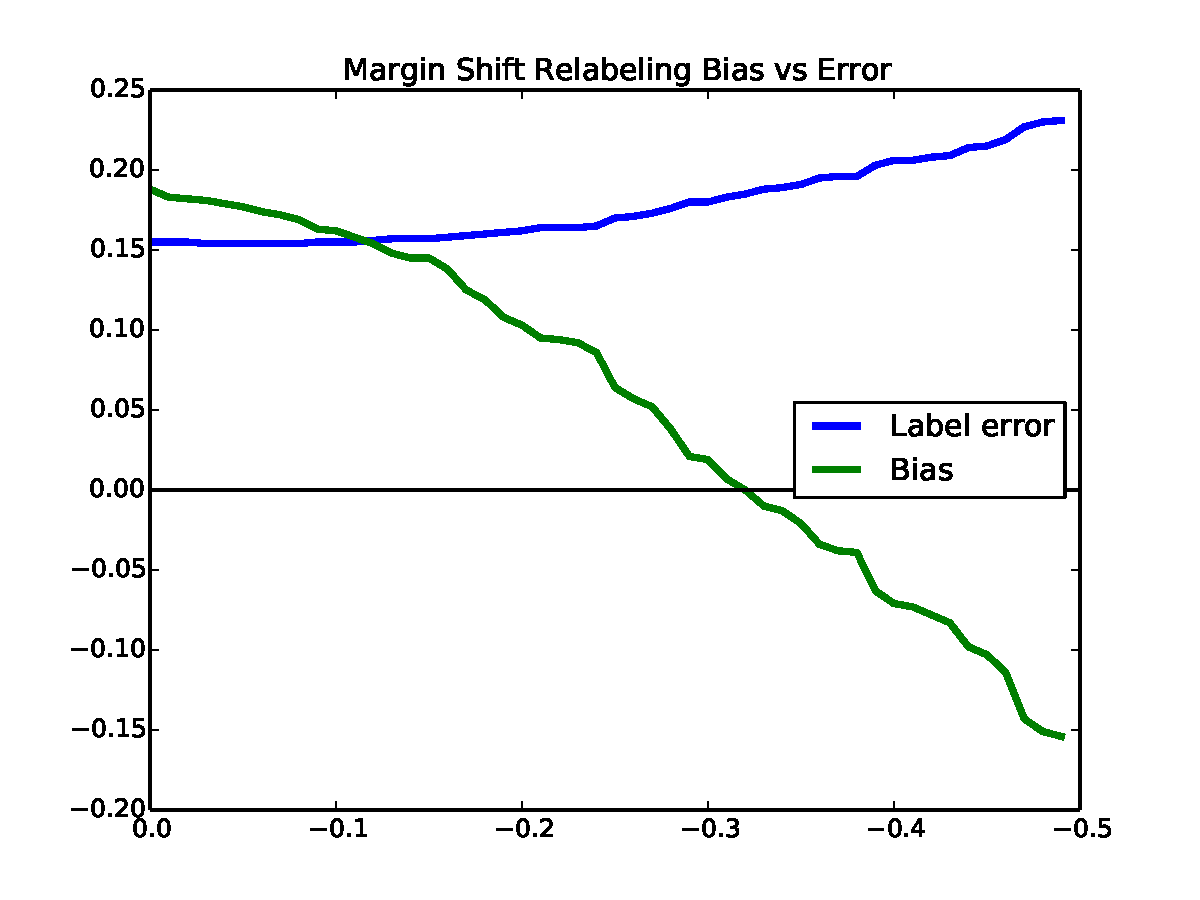
\includegraphics[width=\columnwidth]{images/relabeling-msr-tradeoffs.pdf}
%\caption{Trade-off between (signed) bias and error for SDB. The
%horizontal axis is the threshold used for SDB.}
%\label{fig:tradeoffs}
%\end{figure}
\clearpage

\begin{figure*}[t]
\centering
\begin{subfigure}{.7\columnwidth}
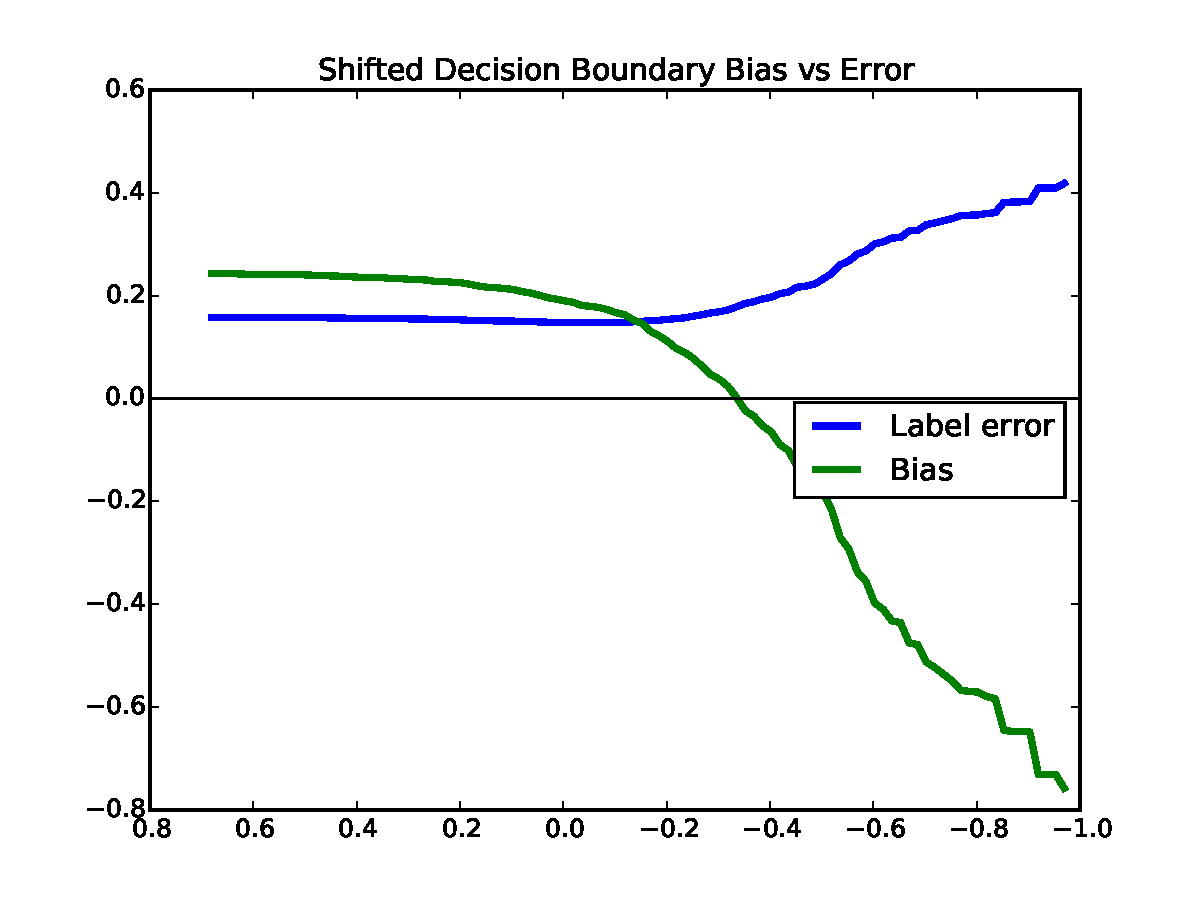
\includegraphics[width=\columnwidth]{images/adult-boosting-T.pdf}%
\caption{Boosting}%
\label{fig:adult_boosting_tradeoff}%
\end{subfigure}%\hfill
\begin{subfigure}{.7\columnwidth}
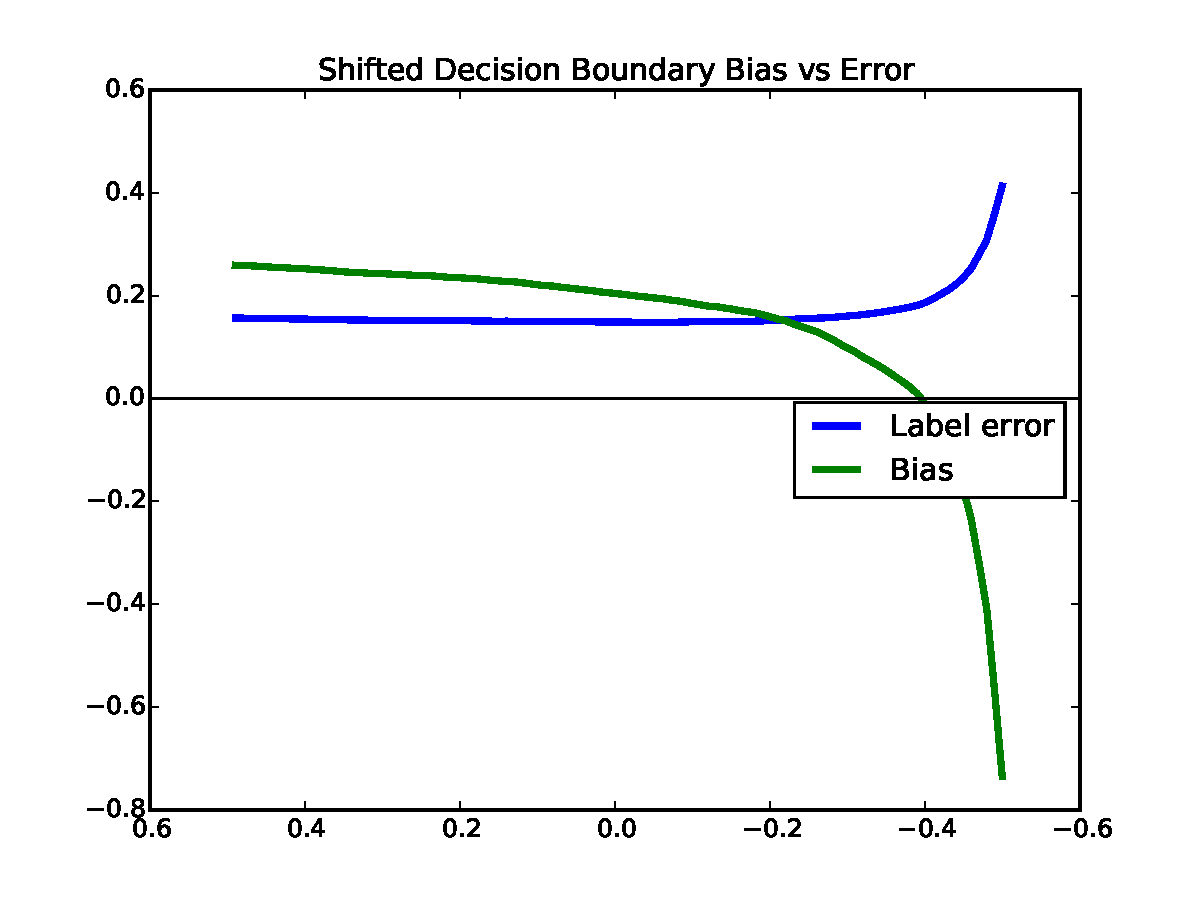
\includegraphics[width=\columnwidth]{images/adult-lr-T.pdf}%
\caption{Logistic Regression}%
\label{fig:adult_lr_tradeoff}%
\end{subfigure}%\hfill%
\begin{subfigure}{.7\columnwidth}
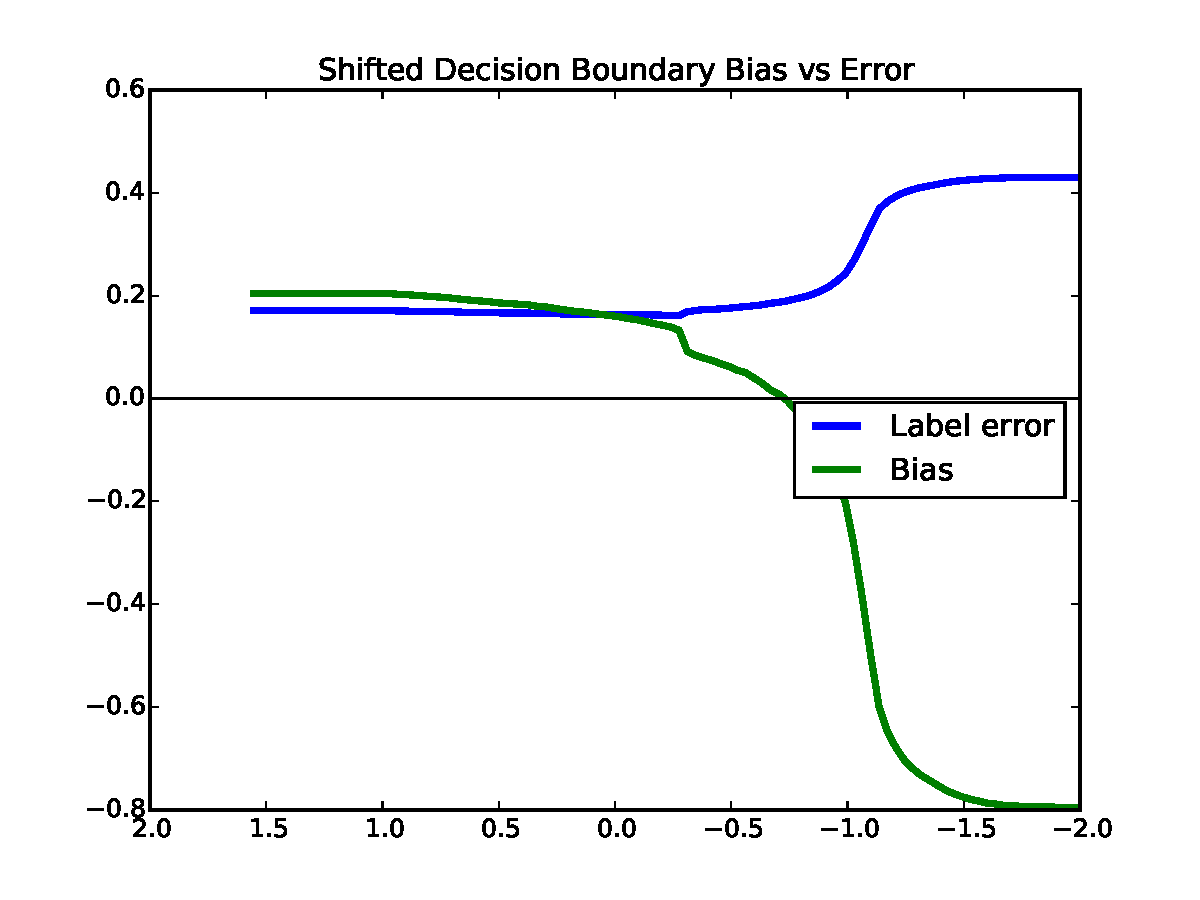
\includegraphics[width=\columnwidth]{images/adult-svm-T.pdf}%
\caption{SVM}%
\label{fig:adult_svm_tradeoff}%
\end{subfigure}%
\caption{Trade-off between (signed) bias and error for SDB on the Census Income data. The horizontal axis is the threshold used for SDB.}
\label{fig:adult_tradeoffs}
\end{figure*}

\begin{figure*}[t]
\centering
\begin{subfigure}{.7\columnwidth}
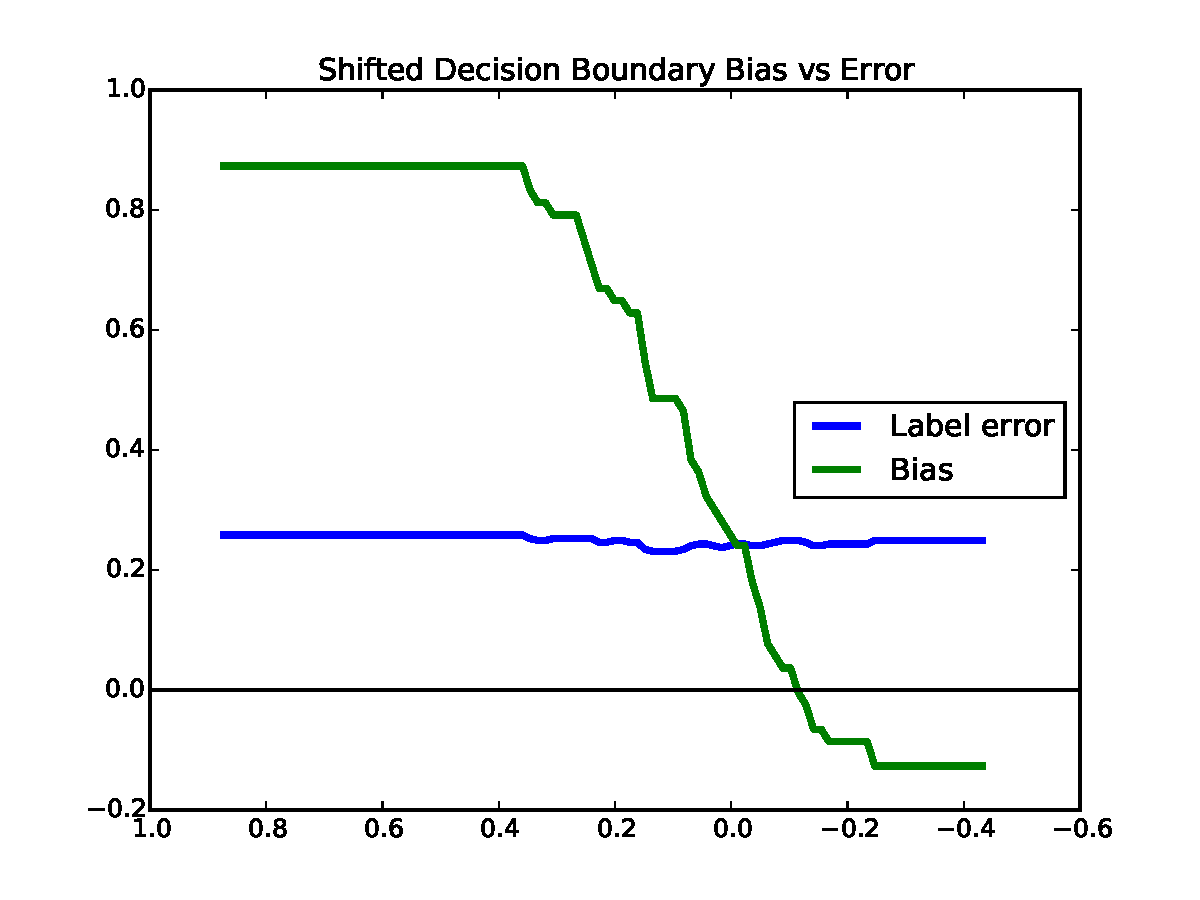
\includegraphics[width=\columnwidth]{images/german-boosting-T.pdf}%
\caption{Boosting}%
\label{fig:german_boosting_tradeoff}%
\end{subfigure}%\hfill
\begin{subfigure}{.7\columnwidth}
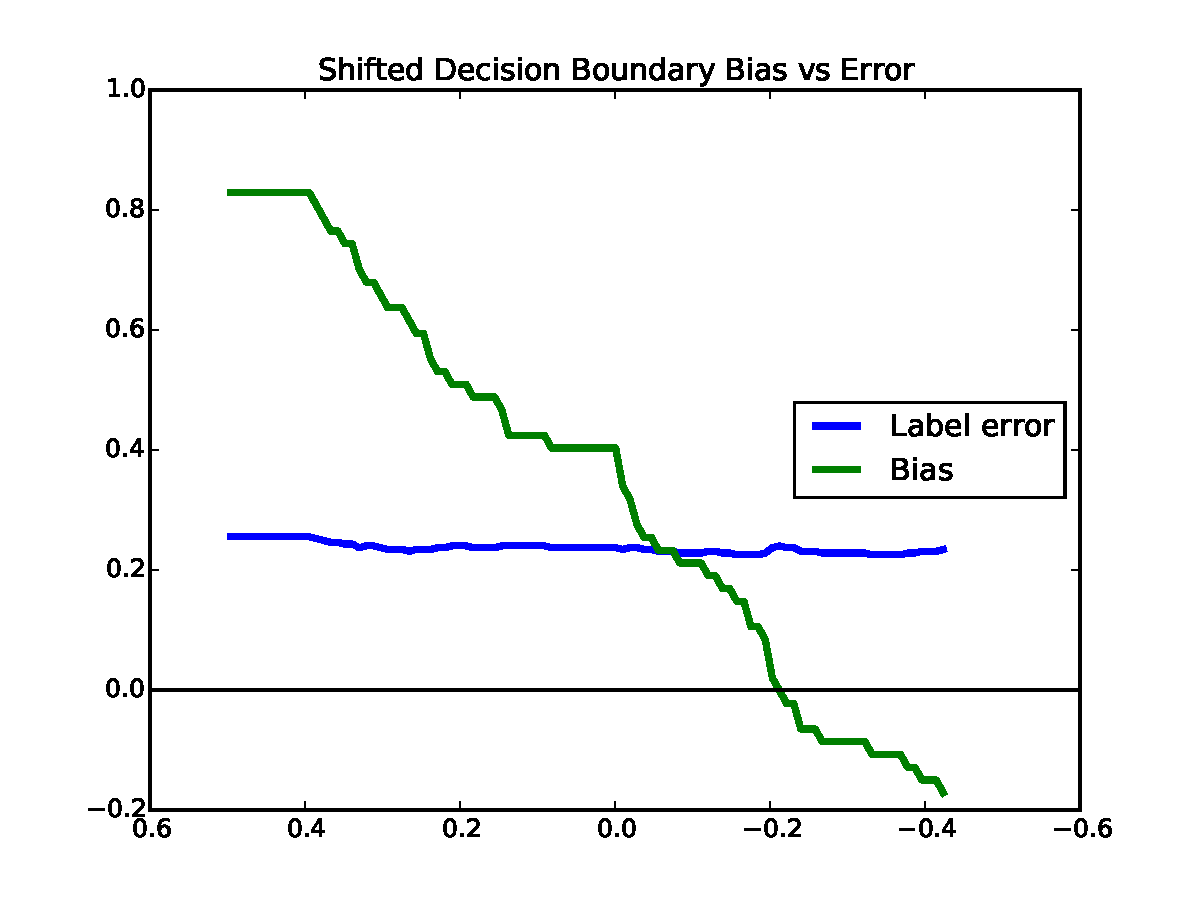
\includegraphics[width=\columnwidth]{images/german-lr-T.pdf}%
\caption{Logistic Regression}%
\label{fig:german_lr_tradeoff}%
\end{subfigure}%\hfill%
\begin{subfigure}{.7\columnwidth}
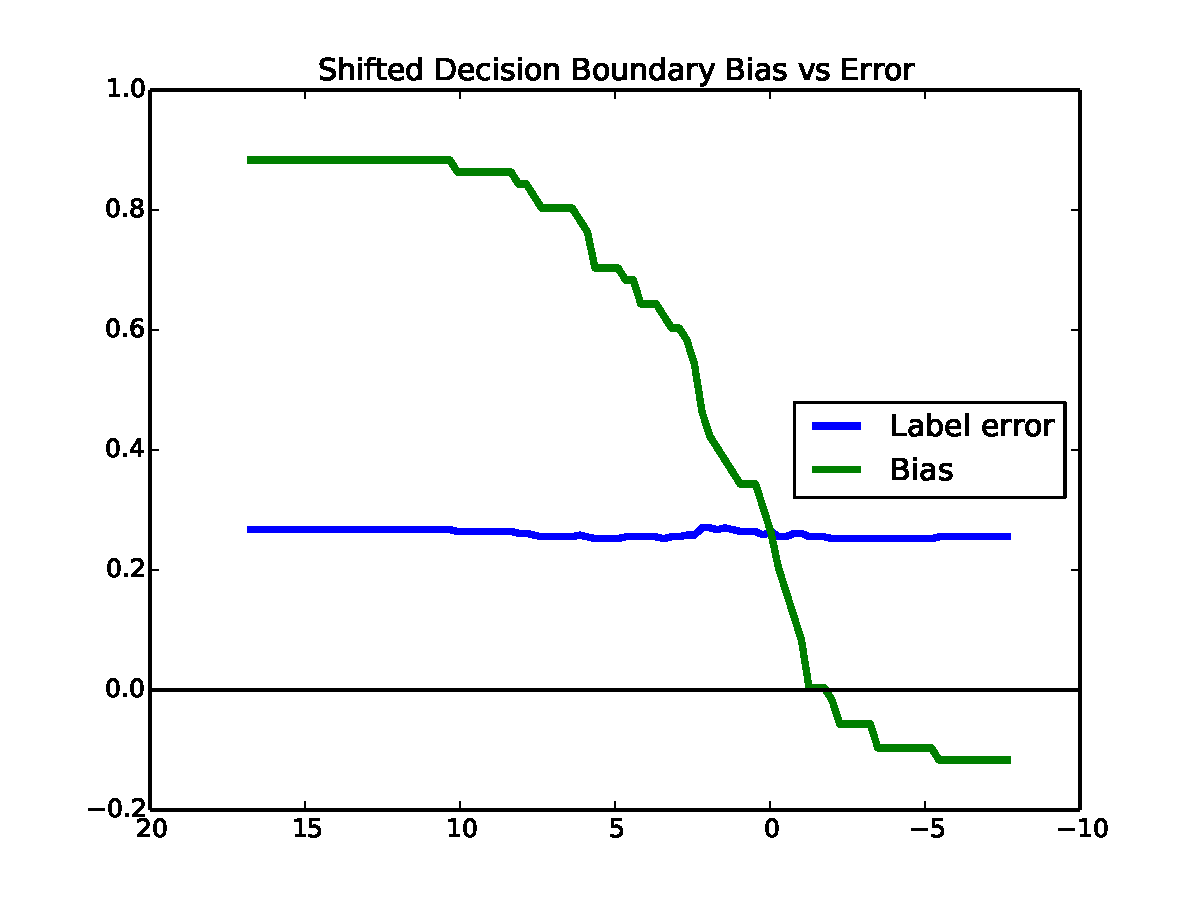
\includegraphics[width=\columnwidth]{images/german-svmlinear-T.pdf}%
\caption{SVM}%
\label{fig:german_svm_tradeoff}%
\end{subfigure}%
\caption{Trade-off between (signed) bias and error for SDB on the German data. The horizontal axis is the threshold used for SDB.}
\label{fig:german_tradeoffs}
\end{figure*}

\begin{figure*}[t]
\centering
\begin{subfigure}{.7\columnwidth}
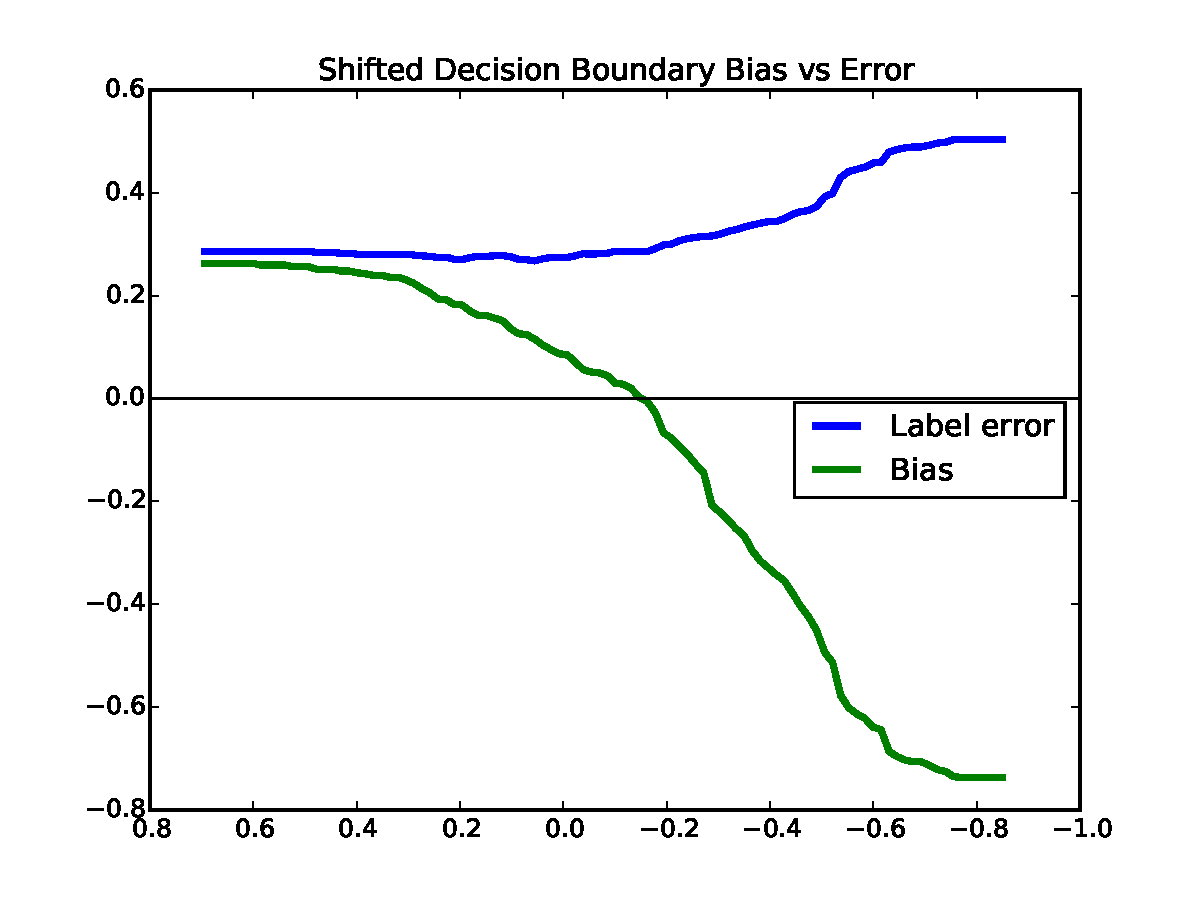
\includegraphics[width=\columnwidth]{images/singles-boosting-T.pdf}%
\caption{Boosting}%
\label{fig:singles_boosting_tradeoff}%
\end{subfigure}%\hfill
\begin{subfigure}{.7\columnwidth}
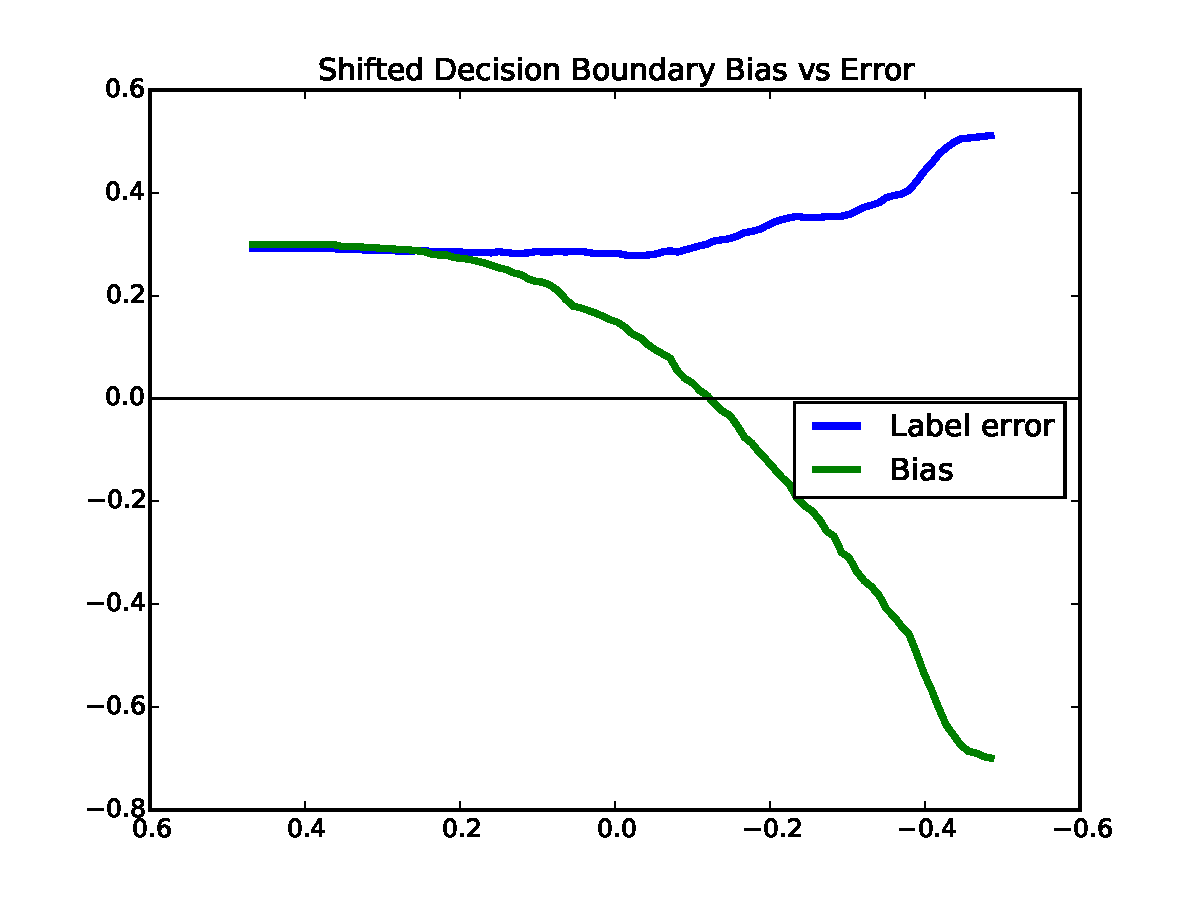
\includegraphics[width=\columnwidth]{images/singles-lr-T.pdf}%
\caption{Logistic Regression}%
\label{fig:singles_lr_tradeoff}%
\end{subfigure}%\hfill%
\begin{subfigure}{.7\columnwidth}
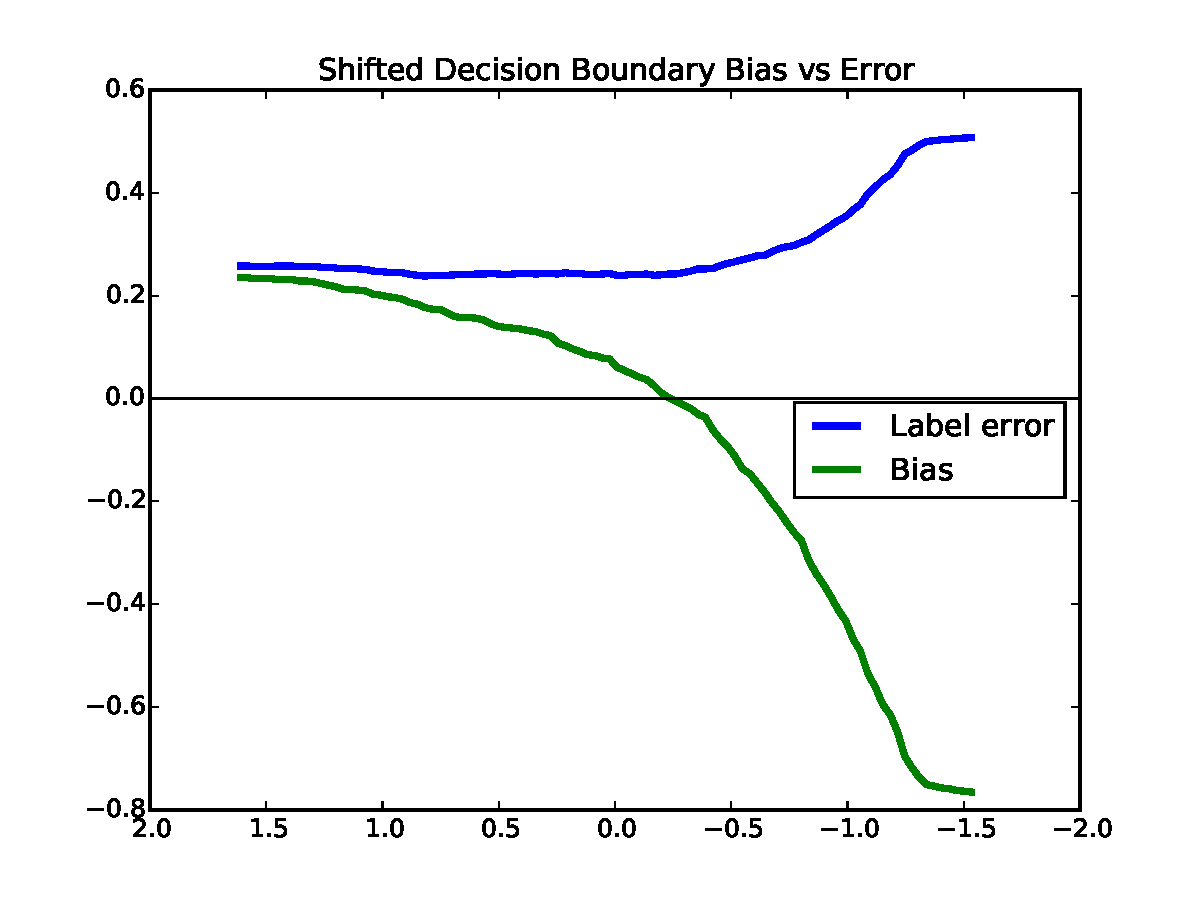
\includegraphics[width=\columnwidth]{images/singles-svm-T.pdf}%
\caption{SVM}%
\label{fig:singles_svm_tradeoff}%
\end{subfigure}%
\caption{Trade-off between (signed) bias and error for SDB on the Singles data. The horizontal axis is the threshold used for SDB.}
\label{fig:singles_tradeoffs}
\end{figure*}

\clearpage



\newpage
\bibliographystyle{IEEEtran}
\bibliography{main}

\end{document}
\grid
